\documentclass[10pt,letterpaper]{article}
\usepackage[margin=0.85in]{geometry}
\usepackage{amsmath,amssymb,booktabs,graphicx,tabularx,array}
\usepackage[numbers,sort&compress]{natbib}
\usepackage{xurl}
\usepackage[hidelinks]{hyperref}
\usepackage{enumitem}
\setlength{\emergencystretch}{1em}
\setlength{\parskip}{3pt}
\setlength{\parindent}{0pt}
\setlist{nosep,leftmargin=*}
\renewcommand{\topfraction}{0.90}
\renewcommand{\bottomfraction}{0.85}
\renewcommand{\textfraction}{0.08}
\renewcommand{\floatpagefraction}{0.85}
\setcounter{topnumber}{3}
\setcounter{totalnumber}{4}
\title{Beyond Recall: Failure Semantics of Long-Term Memory in LLM Agents}
\author{Aditya Mantri\thanks{Independent research. Author background: AI Engineer at Genies; M.S. in Engineering, Purdue University.}\\Independent Researcher}
\date{October 29, 2026}
\begin{document}
\maketitle
\begin{abstract}
Memory mutation recovery involves several obligations that a final fact set cannot distinguish. Stable record addresses can suppress duplicate rows without preserving a chosen decision, while replaying a retained decision can preserve a selected final state and still repeat store operations. We present an independent synthetic factorial study of stable effect addresses, durably retained decisions with target bindings, and completion receipts. All eight policies share the same source and generation frontend; decision retention is identical under both receipt settings. A standalone standard-library implementation uses separate SQLite coordinator and effect stores, fresh Python subprocesses, abrupt exits at declared semantic barriers, unavailable mutation responses, and coordinated generation resets. The primary campaign contains 528 unique structural runs, 928 process attempts, and 256 abrupt terminations. Content correctness, physical cardinality, acknowledgement, decision continuity, planning invocations, and committed put/delete calls are observed separately. With neither stable addresses nor retained decisions or receipts, 42 of 66 runs have correct contents but only 29 satisfy the selected terminal conjunction. Retained decisions without stable addresses produce 66 content passes but 37 terminal passes. Stable addresses with retained decisions produce 66 terminal passes under either receipt setting; receipts reduce committed put/delete calls from 317 to 275 without changing the 66 planning invocations. Five additional probes delimit metadata retention, preparation, and intervening-write assumptions. Independent checking and same-host reproduction in a second Python/SQLite environment agree with the primary outcomes. The contribution is a transparent conformance artifact and measured mechanism distinctions, not a new recovery algorithm or evidence of live-model memory quality.
\end{abstract}
\section{Introduction}
\label{sec:introduction}

Long-term memory lets an agent carry information from one interaction into another. Systems that retain conversational facts, revise stored knowledge, or organize experiences make memory an evolving state rather than a fixed retrieval corpus \cite{packer2023memgpt,zhong2023memorybank,chhikara2025mem}. An update to that state also has an execution history: a decision is chosen, records are written or deleted, and completion is reported. An interruption can separate those events, while a repeated delivery can execute part of the history again.

The resulting questions extend beyond whether an agent can recover the expected fact. A repeated insertion can preserve the fact set while creating additional physical records. A stable record address can suppress those extra records while allowing a newly chosen value to replace the original decision. Conversely, replaying a retained decision through stable writes may preserve the selected final state without a completion receipt, while still issuing additional store operations. These are distinct observations, and whether each constitutes a failure depends on the declared contract. A content oracle, an operation count, and a terminal acknowledgement should therefore not be treated as interchangeable measures.

Neither the recovery mechanisms nor the need to evaluate more than recall is new. RIFL separates request identity, completion records, retry routing, and safe reclamation; Beldi uses logged replay for stateful serverless workflows \cite{lee2015implementing,zhang2020fault}. LIMBO grades ambiguous writes against committed effects, and Permission to Retry separates recovery evidence from authority and unresolved outcomes \cite{li2026where,marla2026permission}. TimlMemBench and prospective-memory evaluation already examine lifecycle and governed-use failures that factual answering can conceal \cite{zhou2026timlmembench,bilgin2026capture}. These predecessors motivate a narrower empirical question: what distinctions become visible when stable effect addresses, retained decisions, and terminal receipts are varied independently under the same memory-mutation contract?

We specify an independent factorial artifact that exposes those three mechanisms as separate controls. All variants share the same synthetic conversation frontend, operation profiles, and controlled decision tape. When decision persistence is enabled, the selected decision remains available after success under both receipt settings; the receipt comparison therefore does not change decision retention. Separate local databases hold recovery state and the record ledger. Each attempt runs in a fresh process, with abrupt termination at declared semantic barriers, unavailable put/delete responses, and coordinated resets. Additional probes examine loss of retained recovery information, interruption before a decision is stored, and an intervening external write. The design asks which obligations each mechanism addresses rather than assuming that every mechanism is necessary for every outcome.

The artifact distinguishes exact fact-set correctness, physical cardinality, final acknowledgement, per-intent decision continuity, planning invocations, and committed put/delete calls. Its selected terminal conjunction covers only the first three observations. It does not certify preservation of a later writer, transient-read isolation, linearizability, or the truth of a retained decision. The contribution is the explicit factorial specification and independently implemented evidence structure for measuring these distinctions. It is an application of established recovery ideas, rather than a new recovery algorithm. Controlled decisions and local stores make the execution question inspectable while leaving live-model quality, natural decision-drift frequency, adversarial memory security, and production behavior outside the study.

\section{Related Work}
\label{sec:related-work}

\subsection{Memory Representation and Lifecycle Evaluation}
Memory architectures establish several ways to retain and revise information across interactions. MemGPT manages memory tiers, MemoryBank combines persistent memory with updating and forgetting, and Mem0 provides conversational extraction and consolidation \cite{packer2023memgpt,zhong2023memorybank,chhikara2025mem}. A-MEM, Zep, Hindsight, and MemOS explore linked, temporal, retention-oriented, or operating-system abstractions for agent memory \cite{xu2025amem,rasmussen2025zep,latimer2025hindsight,li2025memos}. These works make memory management and mutation existing research subjects. Our operation tape controls the selected mutations so that recovery behavior can be examined independently of the quality of the representation or selection policy.

Content and use benchmarks address capabilities that this control deliberately removes. LoCoMo and LongMemEval evaluate long-term conversational memory, including reasoning over prior interactions and changing information \cite{maharana2024evaluating,wu2024longmemeval}. MemoryAgentBench examines memory through incremental interactions; HaluMem studies hallucinations across memory operations; UTILMEM evaluates utilization of distributed and noisy evidence \cite{hu2025evaluating,chen2025halumem,qing2026utilmem}. Exact synthetic facts do not substitute for those semantic evaluations. In particular, a correct terminal fact set in the present artifact is not a measurement of question-answering accuracy or retrieval recall.

Lifecycle and governed-use evaluations are closer to the motivation. TimlMemBench separates a canonical-pool question-answering control from raw-session ingestion and cases involving revocation, supersession, scope, provenance, boundaries, activation, and restraint \cite{zhou2026timlmembench}. \emph{Capture Is Easy, Forgetting Is Hard} evaluates standing constraints with distinct release authorities and an explicit-operation alternative to replacing the whole pin board \cite{bilgin2026capture}. Memora evaluates conversational memory consolidation and mutation, using FAMA to penalize obsolete information in responses \cite{uddin2026memora}. Our standalone factorial study measures execution mechanisms and physical effects under controlled faults, complementing that semantic-validity question. Thus, evaluation beyond recall and the importance of correct forgetting are prior work. The present specification instead varies execution mechanisms underneath a controlled mutation policy; it does not introduce a population-level conversational benchmark or demonstrate better semantic memory management.

\subsection{Logged Recovery, Transactions, and Completion Evidence}
Distributed execution already distinguishes successful return from uncertain failure. Birrell and Nelson's RPC semantics leave the caller uncertain after a failure even though a successful return establishes execution \cite{birrell1984implementing}. RIFL combines unique request identifiers, durable completion results, retry rendezvous, and reclamation that respects acknowledgements and client validity \cite{lee2015implementing}. Crucially, its completion metadata must be atomic with the mutations it describes. Separate commits to an effect ledger and a receipt store do not inherit that guarantee. These foundations make identity, retained results, and recognition lifetime necessary parts of the experimental contract rather than new primitives introduced here.

Beldi provides a close predecessor for retaining nondeterministic results and replaying completed work under its API and storage assumptions \cite{zhang2020fault}. ARIES supplies database-level write-ahead recovery and recorded redo/undo \cite{mohan1992aries}. Persisting chosen operation arguments follows this established distinction between replaying recorded work and recomputing a choice. The independent artifact does not implement ARIES recovery, Beldi transactions, or a guarantee for arbitrary external services; its separate stores and declared operation semantics remain explicit boundaries.

Compensation and effect settlement also have established semantics. Classical sagas repair partially completed long activities through compensating transactions, with application-level compensation distinct from restoring an exact earlier state \cite{garciamolina1987sagas}. SagaLLM applies persistent context, validation, and compensation to agent planning; Atomix separates tool execution from settlement using effect classes and resource progress; Agentic Transaction considers semantic transaction properties, including memory \cite{chang2025sagallm,mohammadi2026atomix,sun2026agentic}. These approaches are conceptual predecessors, not experimentally defeated baselines. A terminal state check in the present study establishes neither transactional isolation nor atomic visibility across stores, and a compensated or repeated operation remains part of its execution history.

\subsection{Fault Histories and Recovery Conformance}
Agent-specific recovery work already studies divergence and uncertain effects. ACRFence validates post-restoration action replay and authority resurrection, while proposing an effect-log analyzer with replay-or-fork semantics that was not implemented in that evaluation \cite{zheng2026acrfence}. LIMBO supplies deterministic service contracts and effect-ledger grading across models and harnesses, explicitly including ambiguous writes, late commits, redelivery, and partial batches \cite{li2026where}. Permission to Retry evaluates authored policies on native persistence hosts and distinguishes retained observations, authority, completed work, and unresolved obligations \cite{marla2026permission}. These works precede the general fault families and much of the conformance methodology used to motivate the independent artifact.

Systematic fault selection also has a substantial foundation. Lineage-driven fault injection reasons from successful outcomes to candidate failures under an explicit bounded system model \cite{alvaro2015lineage}. The manually authored histories here do not implement that search or establish exhaustive coverage, even within a bounded state space. Their purpose is to expose selected interactions among address stability, decision retention, and receipts while holding the surrounding frontend fixed. Receipt removal and an intervening write are boundary questions, not grounds for a universal exactly-once claim. Likewise, committed put/delete counts are separate observations from final state and should not be interpreted as automatically invalid whenever they exceed the count of distinct desired facts.

\subsection{Adversarial Memory Contents}
Execution correctness is complementary to the trustworthiness of stored information. AgentPoison studies poisoned memory or knowledge demonstrations under insertion and embedder assumptions; MINJA induces malicious records through query-only interaction under its retrieval and shared-memory setting \cite{chen2024agentpoison,dong2025memory}. Neither threat is resolved merely by replaying a chosen decision faithfully. The present synthetic frontend defines operational eligibility and controlled decision variation. It does not establish that accepted contents are benign, isolate users against an attacker, evaluate either poisoning attack, or provide a defense against them.
\section{Contract and Mechanism Factors}
\label{sec:contract}

\subsection{Logical intent, attempts, and eligible source}
A logical intent denotes the memory update to recover, whereas a process attempt denotes one execution of that update. Let $j$ be the stable intent identifier and $a$ an attempt index. Each structural run has one fixed $j$ and isolated stores; a retry changes $a$ while retaining $j$. The artifact does not test an identifier-allocation service, overlapping intents, or a population of concurrent agents. This separation lets the experiment vary record addressing and completion recognition without also changing the input identity.

The common source frontend defines the eligible facts before planning. For source endpoint $e$ and expected generation $g$, let $H_{e,g}$ be the ordered conversation rows satisfying the enabled predicate, generation equality, and endpoint bound. The implemented query selects enabled rows with the expected generation and turn at most $e$, ordered by turn. The controlled planner retains the latest selected fact for each attribute. The main fixture uses $e=1$ and $g=0$; additional future or disabled rows make the source controls discriminating. Removing either corresponding predicate changes the selected topic in its control case.

A chosen decision is an ordered sequence of operations with explicit arguments and target bindings:
\begin{equation}
P_j^{(a)}=\Pi(H_{e,g},\rho,\xi_a)
        =(p_0,\ldots,p_{m-1}),
\qquad p_i=(\mathrm{kind}_i,\mathrm{fact}_i,\mathrm{target}_i).
\label{eq:decision}
\end{equation}
Here $\rho$ is the operation profile and $\xi_a$ is the controlled decision-tape choice. A put may insert a new record or revise a named existing target; a delete names its target. The planner does not call a language model, retrieve semantically similar memories, or infer targets from an evolving store. Prescribed changed-tape retries replace \texttt{topic=cycling} with \texttt{topic=running}. This explicit variation isolates recovery of a choice from the probability or quality of naturally generated choices.

\subsection{Three independently varied mechanisms}
The D factor controls addresses for targetless puts, independently of decision retention. If an operation already names an existing target, that binding is used under both D settings. Otherwise D1 derives a deterministic address from $(j,i)$, and D0 generates a fresh address each time the operation is applied. Concretely, D1 uses the first 24 hexadecimal characters of SHA-256 over the intent and instruction slot; D0 uses a fresh 12-byte random value represented in hexadecimal. The experiment evaluates these address rules, not cryptographic collision probabilities. A stable slot address identifies where an operation writes; it does not fix the value that a replanned operation writes there.

The P factor controls whether the selected decision is durably retained. P1 commits the literal ordered operations, including target bindings, to the coordinator before applying effects, then loads that decision on later attempts. P0 chooses again whenever it reaches planning. A retained decision contains targetless puts as targetless operations: D0 still assigns fresh insertion addresses when it replays them. Thus P1 can preserve the chosen facts and targets while allowing duplicate physical insertions. This construction separates decision continuity from effect-address stability instead of embedding one in the other.

The R factor controls a terminal receipt and its fast path. R1 checks a retained receipt after the entry generation check and, on a hit, acknowledges the recorded outcome without reapplying the decision. Successful finalization stores that receipt after effect processing. R0 performs neither receipt lookup nor receipt storage. Crucially, a P1 decision remains stored after success under both R0 and R1. The receipt comparison therefore holds plan retention fixed. It can reveal a reduction in repeated committed operations even when retained decisions and stable addresses already preserve the selected final state.

\subsection{State, decision, and work observations}
The selected terminal contract combines three explicitly limited observations. Let $\mathcal R$ be the multiset of terminal physical records, $E$ the expected set of fixture facts, and $\phi(r)$ the fact in record $r$. Let $A$ hold when the final process exits normally with an acknowledgement event. Define
\begin{align}
C(\mathcal R,E)&\equiv\{\phi(r):r\in\mathcal R\}=E,\label{eq:content}\\
K(\mathcal R,E)&\equiv|\mathcal R|=|E|,\label{eq:cardinality}\\
T(\mathcal R,E,A)&\equiv C(\mathcal R,E)\land K(\mathcal R,E)\land A.\label{eq:terminal}
\end{align}
$C$ intentionally collapses identical duplicate facts, while $K$ inspects physical row count. Neither observes semantic truth, question-answering accuracy, or retrieval recall. $T$ is a selected terminal conjunction for a specified history, not a certificate for all recovery properties.

Decision continuity is a separate per-intent observation. If $\mathcal D_j$ is the set of digests of decisions reported as chosen or loaded for intent $j$, the recorded continuity check is
\begin{equation}
L\equiv\bigwedge_j\bigl(|\mathcal D_j|\leq1\bigr).
\label{eq:continuity}
\end{equation}
The checker recomputes chosen-decision digests from their operation arguments and groups observations by intent. It does not add $L$ to $T$. Moreover, a chosen decision reported before durable preparation is still an observation for $L$; a later change at that boundary does not violate a claim restricted to an already stored decision. Digests summarize observed decisions, not unobserved computation or a security proof.

Committed work is observed independently of both state and continuity. We count planning invocations from decision-chosen events and committed effect calls $W$ from the effect-store audit, one row per participant put or delete commit. Repeated deletion of an absent target is still a committed call. $W$ excludes reset and cleanup SQL mutations, reads, coordinator writes, plan and receipt I/O, tokens, monetary cost, and latency. Extra calls are evidence of repeated work under this definition; they are not automatically an incorrect final state or an unlawful external effect.
\section{Independent Implementation and Failure Model}
\label{sec:implementation}

\subsection{State layout and commit boundaries}
The implementation is a standalone Python standard-library program with two separately committed SQLite files. The coordinator stores the synthetic conversation, current generation, retained decisions, and optional receipts. The effect store holds addressed memory records tagged with intent and generation, plus a committed-action audit. The participant never reads that audit to decide whether an operation already happened; an external evaluator reads it after execution. Figure~\ref{fig:architecture} shows these roles and distinguishes controlled inputs from executed algorithms, storage, and process control.

A put and its audit insertion commit together inside the effect-store connection; a delete and its audit insertion do likewise. Preparation commits a retained decision in the coordinator, and receipt finalization commits there separately. A reset first commits the new coordinator generation and then performs its effect-store deletion; cleanup is another effect-store transaction. No transaction spans both files, and no store is attached to the other to create a shared commit. The implementation sets \texttt{synchronous=FULL} and \texttt{journal\_mode=DELETE}. These settings and SQLite's documented atomic-commit machinery define local storage behavior; they do not make separately committed application actions atomic across files \cite{sqlite2026atomiccommit}.

The operation profiles make both ordering and target reuse concrete. Insert performs three targetless puts. Revise performs three puts, including a put to the existing unit record. Retire deletes a named retired record and then performs three puts. Mixed performs an existing-target unit put, a targetless tone put, the named delete, and a targetless topic put. Operations execute in that order, each with its own effect-store commit. The effect store supplies declared upsert/delete semantics rather than a vector-search interface. Because the first put in retire follows a delete, a fault after the first put is not generally a fault after the first effect.

\begin{figure}[tbp]
\centering
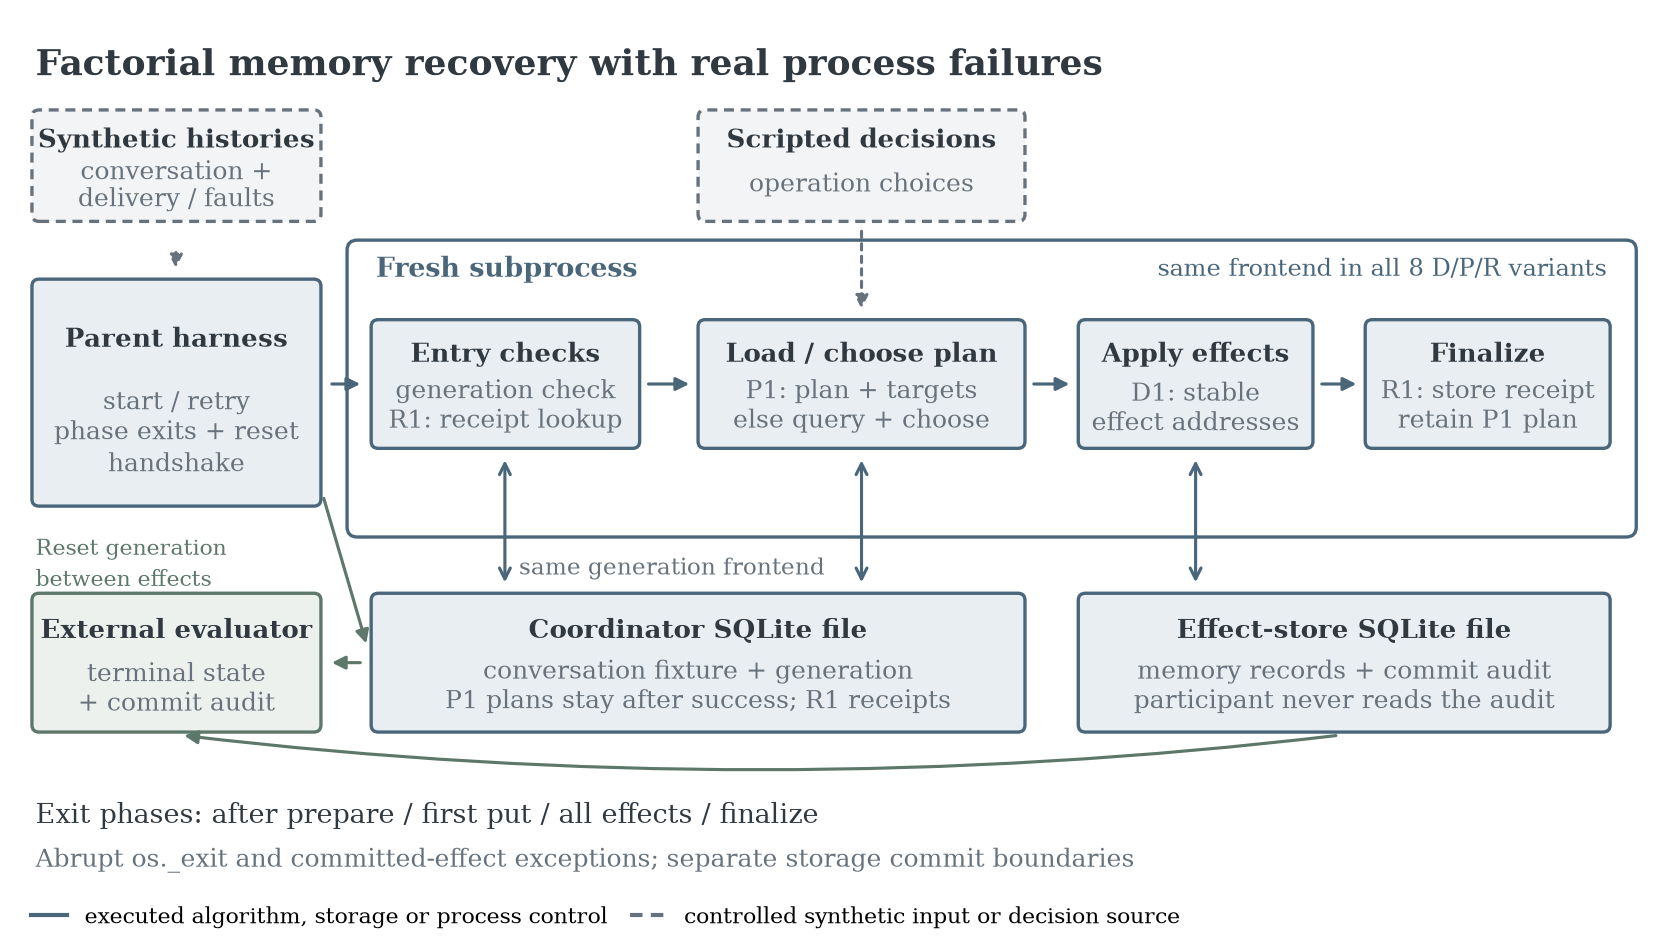
\includegraphics[width=\textwidth]{figures/fig_experiment_architecture.png}
\caption{Independent experiment architecture. A controlled conversation/failure history and decision tape feed a common frontend across all eight combinations of stable effect addresses (D), retained chosen plans with target bindings (P), and completion receipts (R). Every attempt runs in a fresh Python subprocess. Generation checks precede the receipt fast path; receipt and retained-plan hits bypass the shared source query. The coordinator and effect store use separate SQLite files; the participant does not read the effect-store commit audit. The parent harness schedules abrupt process exits, committed-effect exceptions, and a real generation reset between effects through a handshake. P1 retains its chosen plan after success with either R setting. Dashed boxes identify controlled inputs, while solid boxes identify executed algorithms, storage, and process control. The process frame does not imply an atomic cross-store transaction.}
\label{fig:architecture}
\end{figure}

\subsection{Worker procedure and preparation obligation}
Every attempt starts a fresh subprocess and reopens the two files. Its recoverable information comes from retained database state rather than an in-memory object surviving the previous attempt. The following procedure specifies the implemented order and the places at which the main campaign terminates a process.
\begin{enumerate}[label=\arabic*.]
\item Read the current coordinator generation. If it differs from the intent's expected generation, remove records tagged with that intent and generation, acknowledge cancellation, and return.
\item Under R1, look up a matching receipt. On a hit, acknowledge its stored outcome and return without planning or effects.
\item Under P1, load a retained decision if present. Otherwise run the common enabled/bounded source query, choose the operation tape, and, under P1, commit it with its target bindings. This is the preparation boundary. An exit after preparation can now occur.
\item Execute operations in their retained or newly chosen order. Each put or delete commits its record mutation and audit entry together. A configured exit can occur after the first put; configured unavailable-response exceptions occur after a put or delete has committed.
\item Read the generation again after the operation loop. If it changed, delete this intent's old-generation records and select a cancelled outcome; otherwise select applied. An exit after effects can now occur.
\item Under R1, commit a receipt containing the outcome and decision digest. Keep any P1 decision under either R setting. An exit after finalization can now occur; otherwise emit acknowledgement and exit normally.
\end{enumerate}
Receipt and retained-decision hits bypass the source query, while the query implementation itself is shared by all variants. A process exit before P1's decision commit leaves no durably chosen plan to reuse. The main preparation histories place their barrier after the optional save; an additional before-store probe tests the earlier boundary. Retaining a selected decision follows established logged-replay ideas \cite{zhang2020fault}; the study varies that mechanism without attributing database-level recovery or an external atomic-settlement guarantee to it.

\subsection{Termination, uncertain replies, and resets}
The harness controls fault timing but executes actual process termination. The child emits a flushed barrier witness and calls \texttt{os.\_exit(87)} after preparation, the first put, all effects, or finalization. Python documents this primitive as exiting without normal cleanup handlers or standard-I/O flushing \cite{python2026osexit}. A fresh process then retries against retained files. The barrier is deliberately after the relevant commit has returned: the campaign does not interrupt a SQLite commit, simulate machine power loss, or test a distributed storage failure.

Unavailable responses separate committed effects from successful process return. The child raises a controlled exception immediately after a selected put or delete commit and exits with the failure result. A later attempt may repeat that operation. These histories inspect the distinction between an acknowledged delivery and the effects it left, rather than estimating a provider's failure rate. All variants receive the same schedule and decision-tape setting for each matched structural cell.

Generation reset histories execute real database mutations. Reset-before-retry advances the generation after a first-put exit and retains the intent's residual rows while removing fixture-origin records; entry cancellation must then clean up those residual effects. Reset-between-effects uses a parent/child handshake: after the first put commits, the child waits while the parent commits a new generation and deletes existing effect rows, then resumes the remaining operations. The post-loop generation check removes stale writes produced after that deletion. There is no generation check before every individual mutation. The measured terminal cleanup behavior therefore does not imply uninterrupted atomic visibility to concurrent readers.
\section{Evaluation}
\label{sec:evaluation}

\subsection{Finite campaign and evidence construction}
We organize the experiment around three questions: (RQ1) which errors are hidden by fact-set correctness; (RQ2) how address stability, retained decisions, and receipts interact when retention is held fixed; and (RQ3) which boundaries remain outside a selected terminal pass. These questions concern execution semantics, rather than semantic-response quality.

The campaign crosses 17 specified histories with four operation profiles and eight factorial policies. The lost-delete-reply history excludes the two profiles without deletes, leaving $17\times4-2=66$ structural runs per policy and 528 overall. Each run has isolated stores and a single intent. There are no entity-renaming repetitions or sampled user conversations. The specification and source hash were frozen after development and pilot debugging, before the final campaign; this is neither preregistered nor held-out benchmark construction.

The histories cover ordinary execution; completed redelivery under fixed or changed tapes; exits after preparation, the first put, and all effects under each tape setting; exit after finalization with a changed tape; unavailable put replies under fixed or changed tapes; bounded and disabled-source controls; reset before retry; reset between effects; and unavailable delete replies. The changed tape prescribes a different topic on a later planning invocation. It is a selected adversary for continuity, not a measured natural drift frequency. Figure~\ref{fig:history} gives every history's selected terminal outcome, including partial passes across operation profiles.

The primary environment used Python 3.12.13 and SQLite 3.53.1. The 528 runs required 928 fresh process attempts: 592 normal exits, 256 abrupt exits, and 80 controlled-exception failures. The abrupt exits comprise 64 after preparation, 96 after the first put, 64 after effects, and 32 after finalization. Each policy has 116 attempts and 32 abrupt exits. These attempts are components of the specified histories, not additional independent samples. All final main-campaign attempts acknowledge, so $A$ does not explain the observed differences in $T$.

\subsection{Content, cardinality, and terminal outcomes}
The main results separate facts from their physical representation. Table~\ref{tab:main} reports all eight policies, and Figure~\ref{fig:factorial} displays both oracle counts and execution-work counts. D0P0R0 obtains 42 content passes but only 29 terminal passes. P1 raises content passes to 66 even with D0R0, but physical cardinality still passes in only 37 runs, leaving the same 37 terminal passes. D1P0R0 instead obtains all 66 cardinality passes while content and terminal passes remain 42. The mechanisms preserve different aspects of the selected state.

\begin{table}[tbp]
\centering
\caption{Primary finite campaign, 66 structural runs per policy. $C$, $K$, $T$, and $L$ count passes of the defined content, cardinality, selected terminal, and decision-continuity checks. $Q$ counts planning invocations and $W$ committed participant put/delete calls. All policies acknowledge 66 final attempts. Lower work counts are interpreted within the declared contract, not as generic cost or latency improvements.}
\label{tab:main}
\begin{tabular}{lrrrrrr}
\toprule
Policy & $C\uparrow$ & $K\uparrow$ & $T\uparrow$ & $L\uparrow$ & $Q\downarrow$ & $W\downarrow$ \\
\midrule
D0P0R0 & 42 & 37 & 29 & 42 & 112 & 317 \\
D0P0R1 & 50 & 49 & 41 & 50 & 100 & \textbf{275} \\
D0P1R0 & \textbf{66} & 37 & 37 & \textbf{66} & \textbf{66} & 317 \\
D0P1R1 & \textbf{66} & 49 & 49 & \textbf{66} & \textbf{66} & \textbf{275} \\
D1P0R0 & 42 & \textbf{66} & 42 & 42 & 112 & 317 \\
D1P0R1 & 50 & \textbf{66} & 50 & 50 & 100 & \textbf{275} \\
D1P1R0 & \textbf{66} & \textbf{66} & \textbf{66} & \textbf{66} & \textbf{66} & 317 \\
D1P1R1 & \textbf{66} & \textbf{66} & \textbf{66} & \textbf{66} & \textbf{66} & \textbf{275} \\
\bottomrule
\end{tabular}
\end{table}

A recorded insertion trace exposes the distinction without an aggregate score. In D0P1R0, an exit after the first put leaves one committed tone record. The retained three-put plan replays without replanning, but fresh addresses produce four physical rows for three expected facts, including two copies of \texttt{tone=concise}. Thus $C$ and $L$ hold while $K$ and $T$ fail; four put calls committed. In the changed-tape counterpart with D1P0R0, stable addresses leave three rows but replanning writes \texttt{topic=running}. Here $K$ holds while $C$, $L$, and $T$ fail. D1P1R0 retains the original topic, has three terminal rows, and passes all four checks after the same four committed puts. These statements come from recorded process events and physical rows.

Content-only scoring hides 13, 9, 29, and 17 terminal failures for the four D0 policies in table order. No such gap occurs under D1 in this suite, where acknowledgement is uniform and no excess rows remain. This observed agreement does not make content equality a general terminal-correctness certificate.

\begin{figure}[tbp]
\centering
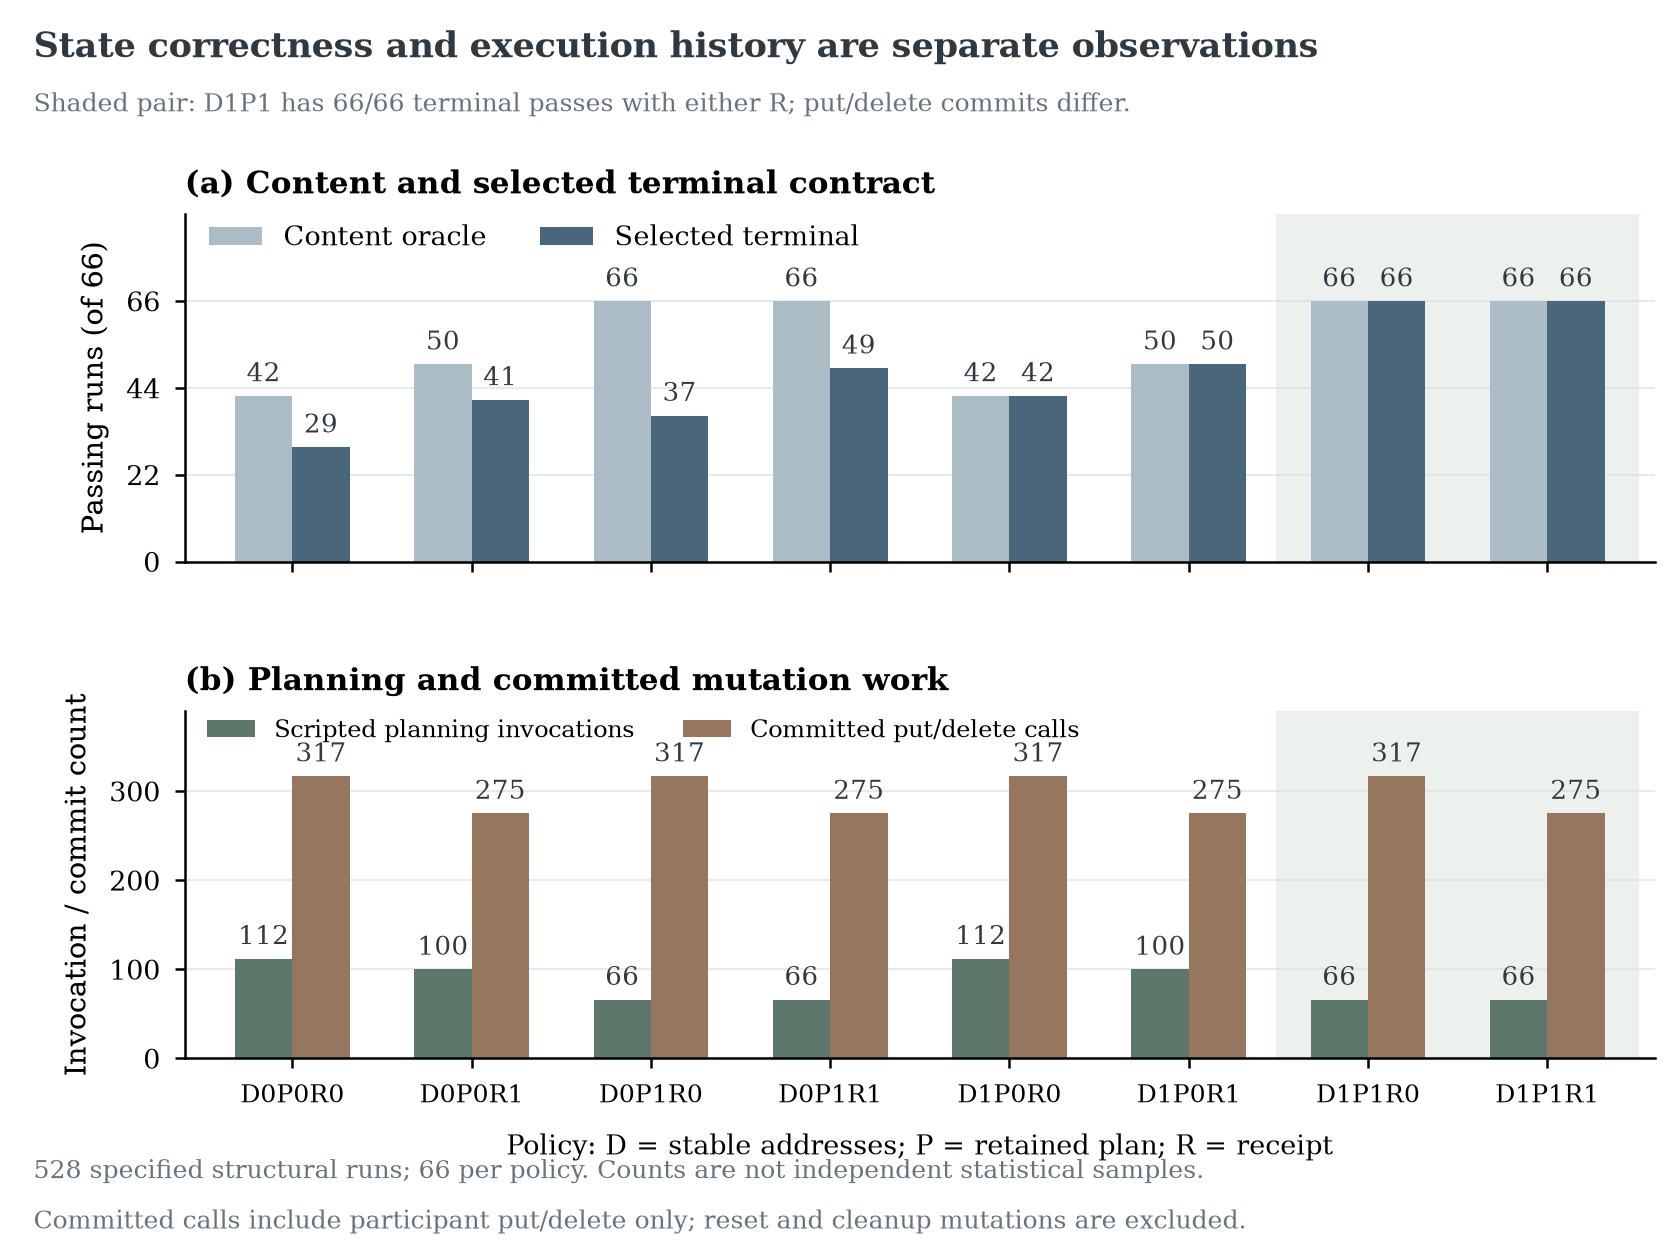
\includegraphics[width=\textwidth]{figures/fig_factorial_oracles.png}
\caption{Content, selected terminal conformance, and execution-work counts for the eight factorial policies. Each policy has 66 specified structural runs. The content oracle checks exact fact-set equality; selected terminal conformance also requires expected physical cardinality and final acknowledgement. The lower panel separately counts scripted planning invocations and committed participant put/delete calls, excluding reset and cleanup mutations. The shaded D1P1 pair passes all 66 terminal checks with either receipt setting while making 317 calls under R0 and 275 under R1. These are finite controlled counts, not population estimates, latency, monetary cost, retrieval recall, or live-model accuracy.}
\label{fig:factorial}
\end{figure}

\subsection{Matched factor contrasts and receipt work suppression}
The complete factorial uses the same frontend, and each D/R comparison holds the P retention rule fixed. Switching D from 0 to 1 yields terminal gains of 13, 9, 29, and 17 runs in the $(P,R)=(0,0),(0,1),(1,0),(1,1)$ strata. Content, continuity, planning counts, and committed-call counts are unchanged by that switch in every stratum. This is consistent with address stability repairing physical replay while leaving both selected decisions and the number of issued mutations unchanged.

Switching P changes the decision observation while leaving effect calls unchanged. It adds 24 content and continuity passes under R0, or 16 under R1, for either D setting. It saves 46 planning invocations under R0 and 34 under R1. Its terminal gains are 8, 8, 24, and 16 in $(D,R)=(0,0),(0,1),(1,0),(1,1)$ order. The smaller gains under D0 show that preserving the decision does not remove the fresh-address duplication problem. These are exact comparisons of matched constructed cells, not estimates of population causal effects.

Receipts are conditionally redundant for the selected terminal state and still reduce committed work. Switching R gives terminal gains of 12, 12, 8, and 0 in $(D,P)=(0,0),(0,1),(1,0),(1,1)$ order. In the D1P1 pair, both policies pass all 66 $T$ and $L$ checks and plan exactly 66 times. R0 nonetheless commits 317 put/delete calls, whereas R1 commits 275: a difference of 42. Retaining the same decision after success under both policies is essential to interpreting this comparison. The improvement is suppression of repeated committed work, with no selected final-state gain in that stratum.

A completed mixed-profile redelivery makes the receipt distinction concrete. The initial attempt performs three puts and one delete. Under D1P1R0, replay loads the same retained plan and commits those four operations again, including a delete of an already absent target. Under D1P1R1, the retained receipt returns the completed outcome without those four additional operations. Both runs preserve the same final contents and cardinality. Accordingly, an excess operation count need not be called a terminal failure, and a terminal pass need not imply that no operation was repeated.

The history matrix locates the limits of each comparison. A receipt helps after completed work or an exit after finalization, but cannot recognize completion at earlier barriers where no receipt exists. P1 preserves the prescribed original decision after preparation, but under D0 may replay insertions to fresh addresses. D1P1 satisfies all declared terminal histories with or without receipts. All policies pass the bounded-input, disabled-source, and reset controls because those frontend and generation mechanisms are shared. Those controls support the exercised implementation and do not estimate a gain from D, P, or R.

\begin{figure}[tbp]
\centering
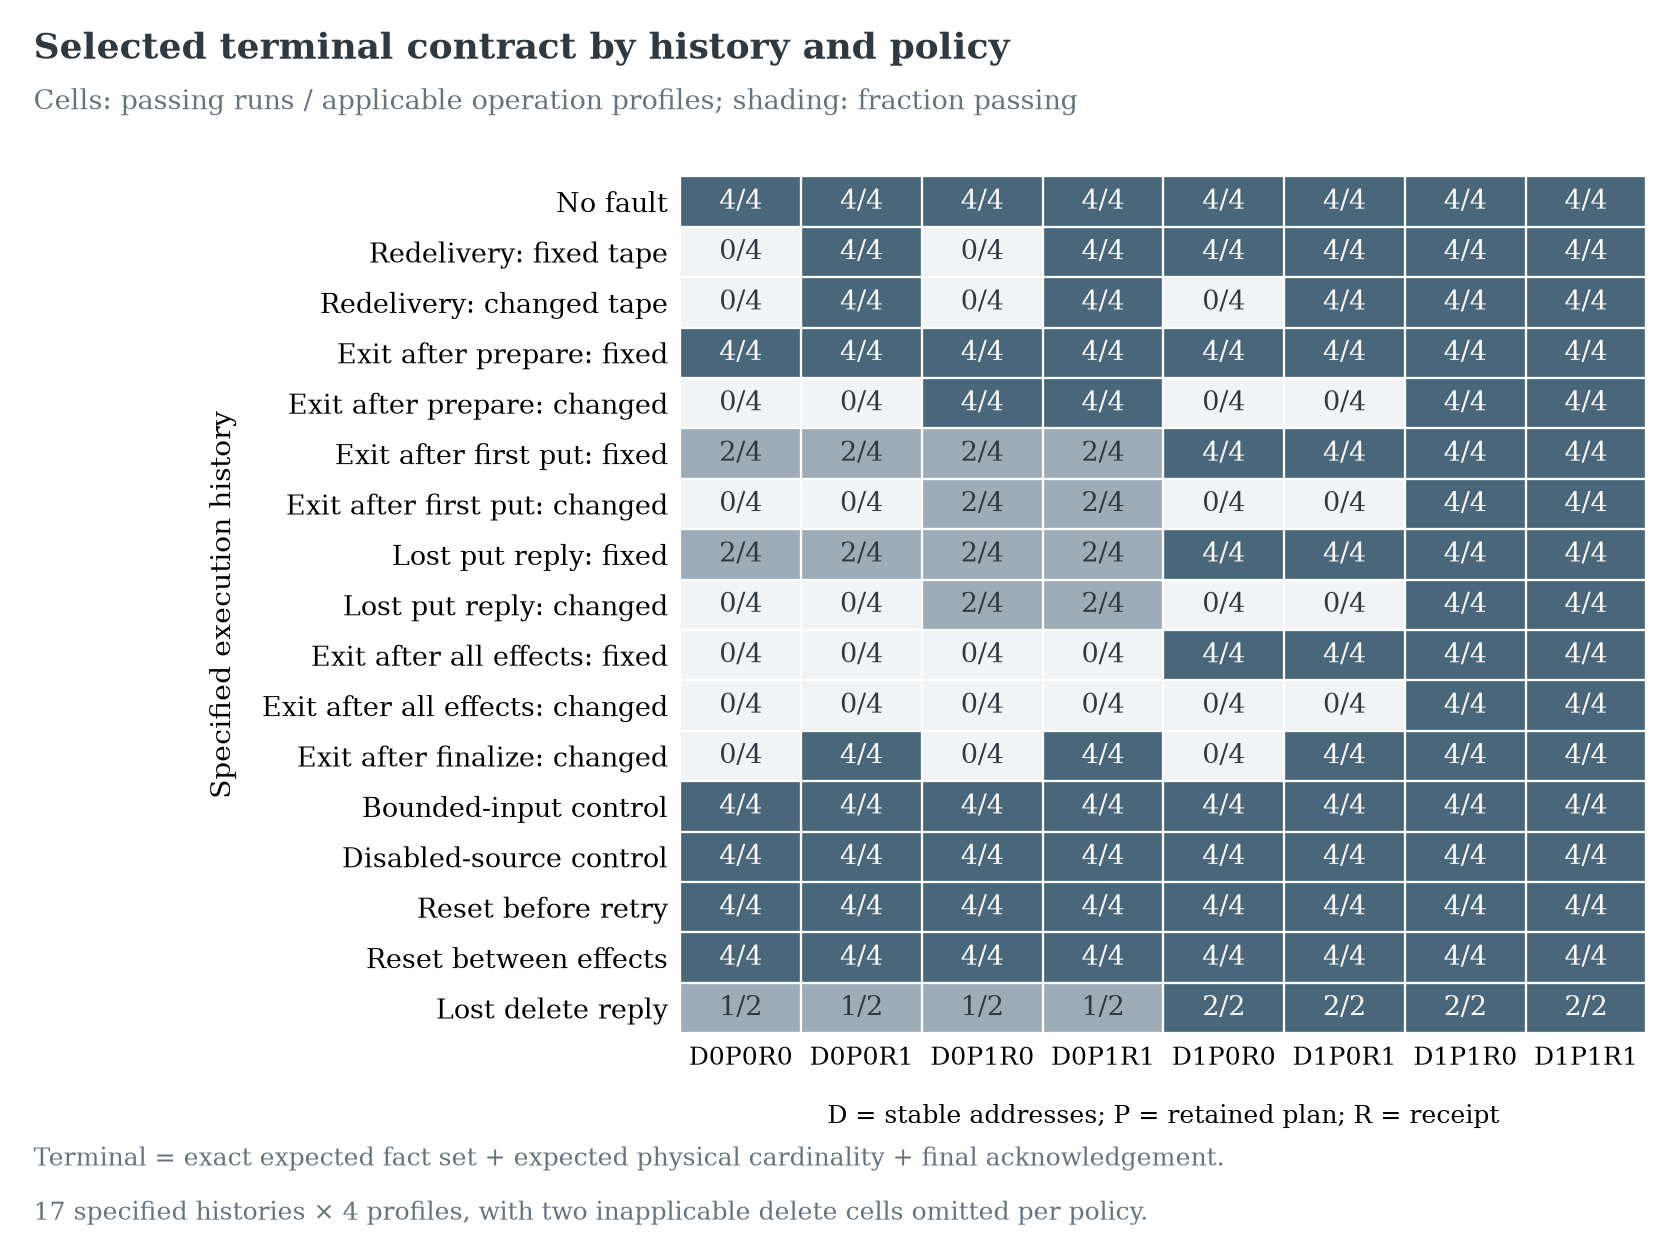
\includegraphics[width=\textwidth]{figures/fig_history_matrix.png}
\caption{Selected terminal conformance by specified history and D/P/R policy. Each cell reports passing structural runs over applicable operation profiles; shading represents that fraction. All histories have four profiles except lost-delete-reply, which has two. Stable addresses, retained decisions, and receipts change different history outcomes. The shared bounded-input, disabled-source, and generation-reset frontend is present in every policy. Changed-tape histories explicitly prescribe a different later decision; their counts do not estimate natural model drift. The matrix covers 528 unique structural runs and does not establish behavior under every process, concurrency, or storage failure.}
\label{fig:history}
\end{figure}

\subsection{Metadata, preparation, and intervening-write boundaries}
Five additional probes retain boundaries that the main success counts do not cover. Table~\ref{tab:boundaries} reports them separately from the 528 structural runs. All use D1P1R1 with the mixed profile and acknowledge their final attempt. The metadata-erasure probes first complete the original decision, then remove the named coordinator state before a changed-tape replay. They are explicit deletion experiments, not tests of a time-based expiration policy.

\begin{table}[tbp]
\centering
\caption{Additional boundary probes under D1P1R1, mixed profile. Pass/fail columns are observations of the specified original-intent checks. $Q$ counts planning invocations and $W$ counts committed participant put/delete calls. The external-write probe passes these checks while losing the newer external value.}
\label{tab:boundaries}
\begin{tabular}{lccccrr}
\toprule
Probe & $C$ & $K$ & $T$ & $L$ & $Q\downarrow$ & $W\downarrow$ \\
\midrule
Remove receipt only & pass & pass & pass & pass & 1 & 8 \\
Remove decision only & pass & pass & pass & pass & 1 & 4 \\
Remove both & fail & pass & fail & fail & 2 & 8 \\
Exit before decision store & fail & pass & fail & fail & 2 & 4 \\
Intervening external write & pass & pass & pass & pass & 1 & 5 \\
\bottomrule
\end{tabular}
\end{table}

Receipt-only deletion preserves the stored decision and all four state/continuity checks, but repeats four mutations for eight total commits. Decision-only deletion preserves the receipt; the fast path suppresses all additional mutations, leaving four total commits and one observed planning invocation. Removing both permits the changed decision: cardinality remains correct, but content, continuity, and terminal conformance fail after eight commits. These observations distinguish evidence that suppresses completed replay from evidence that fixes the operations to replay.

The before-store exit lies outside the prepared-decision obligation. The child reports a chosen decision and terminates before committing it; the next process has no stored decision to load and chooses the changed tape. The resulting $C$, $L$, and $T$ failures demonstrate loss of an uncommitted choice, not failure to reuse a decision already prepared. The recorded continuity metric includes both observed choices, so its failure is expected at this explicitly earlier boundary.

The intervening-write probe demonstrates an important blind spot in the original-intent oracle. After the first put commits and the process exits, an external write changes the existing unit target to \texttt{unit=newer-external-value}. Replay of the retained original decision overwrites it with \texttt{unit=metric}. All four original-intent checks pass with five committed participant calls, but the newer external value is not preserved. This counterexample prevents inferring latest-writer preservation or linearizability from $T$; neither property is specified by that final-state conjunction.

\subsection{Independent checking and software-environment reproduction}
The evidence checker reads archived SQLite state and event traces without importing the participant's metric functions. It recomputes fact-set equality, physical cardinality, final acknowledgement, per-intent decision continuity, planning events, and audit commits, and checks the expected structural keys against the declared coverage. A protocol audit additionally checks retained decisions, target bindings, receipt state, generations, and reconstructed final state. All 528 cases and five boundary probes pass these evidence-consistency checks; the main campaign contributes 688 checked source-selection observations, with probe observations checked separately. This validates correspondence among the retained artifacts and stated finite oracles, not correctness under untested histories.

Ten meaningful standard-library checks pass with zero failures, errors, or skips in each of the two software environments. They cover duplicate-versus-content oracle separation, a real abrupt-exit/resume path, invariant plan retention across receipt settings, finite structural coverage, the unpersisted-decision boundary, rejection of forged metrics, discriminating source controls, the generation handshake, repeated delete calls, and changed decisions under stable addresses. Repeating these checks in both environments does not create 20 unique tests.

A second complete campaign on the same host uses Python 3.14.3 and SQLite 3.51.2. Its 528 freshly created runs, aggregate metrics, and five boundary-probe scalar outcomes match the primary Python 3.12.13/SQLite 3.53.1 campaign with the source hash unchanged. Random fresh addresses may differ, so byte-identical databases are not the equivalence target. This same-host comparison is a software-environment reproduction, not third-party replication or an enlarged main denominator. Separate automated Ubuntu checks are recorded in the artifact provenance. The reported main campaign remains 528 structural runs.
\section{Discussion and Limits}
\label{sec:discussion}

\subsection{What the mechanism separation establishes}
The study makes three recovery observations independently inspectable. Stable addresses can preserve physical cardinality while a changed decision violates the expected facts. Retaining a chosen decision can preserve content and continuity while unstable addresses create extra rows. A completion receipt can suppress repeated committed operations even when it changes neither the selected terminal state nor the number of decisions chosen. The matched D1P1 receipt comparison is especially useful because its plan-retention policy stays fixed. It answers a narrower question than whether a receipt is universally necessary or an algorithm is generally exactly-once.

The contribution is an explicit artifact and finite mechanism analysis built on existing recovery ideas. Unique identities, logged choices, completion evidence, and reclamation already have substantial foundations in RIFL, Beldi, and transaction research \cite{lee2015implementing,zhang2020fault,mohan1992aries}. Governed memory evaluation and effect-side fault grading are also established \cite{zhou2026timlmembench,li2026where}. The present experiment contributes a controlled three-factor decomposition, separate state/decision/work observations, source-visible negative probes, and checked computational evidence. It does not compare empirical performance against those systems or present a new recovery primitive.

\subsection{Assumptions and further evidence needed}
The successful terminal cases rely on a deliberately restricted model. Each run has one fixed intent, known target bindings, isolated local stores, and declared upsert/delete behavior. There are no concurrent participant intents sharing a target, lost or reordered distributed messages beyond the specified schedules, or naturally generated planner decisions. The interposed writer is a negative probe rather than a concurrency workload. Hash-derived addresses identify slots within this model; the study does not establish global identity allocation, cross-user isolation, or collision safety at scale.

Actual abrupt process termination strengthens the process-level evidence while leaving storage-failure assumptions intact. The exits occur after named committed barriers, never midway through SQLite commit. They do not cover power loss, filesystem corruption, remote-provider consistency, or arbitrary asynchronous interleavings. Generation resets are real local operations under a selected handshake, and the post-loop cleanup can leave transient stale rows before it runs. A selected empty terminal state therefore establishes neither atomic forgetting nor the absence of an intervening stale read. Separate effect and receipt commits remain an explicit cross-store gap.

Decision retention protects the choice that was stored, not the correctness or authority of that choice. The before-store and metadata-deletion probes delimit which recovery information remains available, and the external-write probe shows why latest-writer preservation needs its own contract. No clinical task, human judgement, semantic memory truth, live-model QA, retrieval recall, natural drift frequency, memory-poisoning defense, or production reliability is measured. Future work can add multi-intent conflict policies, controlled transient readers, adversarial authority changes, and systematic schedule exploration while keeping these observations distinct. Live-model evaluation would be a separate semantic study rather than a substitute for the operational contract.
\section{Conclusion}
A memory update's fact set, physical records, chosen decision, and committed operation history answer different recovery questions. The independent factorial artifact makes those questions executable under the same source and generation frontend. Across 528 specified structural runs, stable addresses and retained decisions jointly satisfy all 66 selected terminal checks per receipt setting, while receipts reduce put/delete commits from 317 to 275 with no planning-count change. The five boundary probes show why that result depends on retained recovery information and why terminal conformance says little about an intervening writer or an uncommitted choice. Independent checks and a second same-host software-environment campaign reproduce the declared observations. Extending the failure and concurrency model while preserving separate state, decision, and work oracles is the next step; the present evidence remains a finite synthetic mechanism study.
\clearpage
\bibliographystyle{plainnat}
\bibliography{refs}
\clearpage
\appendix
\small
\section{Protocol Specification and Reproducibility}
\label{sec:reproducibility}

\subsection{Commands and artifact structure}
The standalone code, frozen cases, tests, and reproduction evidence accompany this draft at \url{https://github.com/aditya-genies/beyond-recall}. The repository is private at the time of this draft; the link does not assert public access.

The experiment engine and checks use the Python standard library. From the artifact root, the following commands run the focused checks, create a new campaign directory, and independently verify its evidence:
\begin{verbatim}
python3 -W error::ResourceWarning -m unittest -v test_study
python3 study.py campaign --out results_new --workers 4
python3 checks/check_results.py --campaign results_new \
  --out checks/results_new_verification.json
\end{verbatim}
The campaign refuses to overwrite an existing case archive. Each run's directory contains coordinator and effect-store databases; \texttt{cases.jsonl} retains process return codes, barrier witnesses, chosen/loaded decisions, expected facts, physical rows, and committed actions. \texttt{summary.json} aggregates the primary metrics, \texttt{frozen\_spec.json} records the source hash and schedule, and \texttt{boundary\_probes.json} retains the five additional probes. Figure renderers derive their numerical values from checked raw rows and preserve their own input digests. Rendering uses plotting dependencies separate from the standard-library experiment engine.

To reproduce the environment comparison, run the same commands with the Python 3.12.13/SQLite 3.53.1 and Python 3.14.3/SQLite 3.51.2 interpreters into distinct fresh output directories. The retained comparison checks all per-policy aggregate fields and boundary scalar outcomes. Compare those outcomes rather than random insertion addresses or database bytes. The two completed campaigns ran on the same host. Neither the second environment nor repeated unit-check executions changes the main 528-run coverage claim. Automated companion checks also reproduce the complete campaign and five probes on Ubuntu with Python 3.12 and 3.14. Both jobs pass independent verification and match the frozen aggregate outcomes. These additional portability checks are not pooled with the primary coverage.

\subsection{Byte-level evidence pins and coverage}
The final \texttt{study.py} SHA-256 digest is
\begin{verbatim}
98378f217f0dae050dbc07aa04e1121ed9bc73862c2ee35a2e31a7a464f4e9b9
\end{verbatim}
The primary case archive, summary, and frozen specification have these SHA-256 digests, respectively:
\begin{verbatim}
6714681fbefcbdf63334f76b95410aa1c2bc620ce8b7511fadb0c91354b72d01
4d56dceb0a677f6f1bb1d67d037004bf2364080aaf9e03784cbbf5f02cb8ed5f
f5dac100857d093a865b10ff525aaf48fa862f8eb6125cc6771517de6d5c6306
\end{verbatim}
The boundary-probe archive digest is
\begin{verbatim}
f3f02785a6ef5aa91f53bf87e2b604096605831013c06254e64b8f92d4d1d429
\end{verbatim}
These pins identify the exact primary evidence, not a claim that new random-address executions will serialize identically. Relative-path authoring provenance records the manuscript inputs and their hashes separately.

Coverage comprises the declared policy/profile/history product after the two delete exclusions. All final rows, including failures, are retained; probes and reproductions remain separate. Named barriers test recovery between commits under the documented SQLite assumptions \cite{sqlite2026atomiccommit}.

\subsection{AI assistance and provenance}
PaperOrchestra organized the outline, literature review, figures, manuscript drafting, and structural checks \cite{song2026paperorchestra}. AI assistance also supported the standalone experiment, targeted tests, evidence audits, and prose synthesis. Numerical figures derive from frozen raw data checked against the databases and process witnesses. Public-source verification and authoring records accompany the artifact. The author is responsible for the interpretation and release decisions.
\end{document}
